\begin{frame}
\frametitle{高维非线性演化方程多种波解的机械化算法}
\begin{enumerate}
\item 简单 Hirota 方法
\begin{enumerate}
    \item 孤子解
    \item 呼吸子解
    \item lump 解
    \item 相互作用解 
\end{enumerate}
\item 直接代数方法
\begin{enumerate}
    \item lump 解 
    \item 相互作用解 
\end{enumerate}
\end{enumerate}
\end{frame}

\begin{frame}{简单 Hirota 方法的基本流程}
\begin{enumerate}
\item \Painleve{}分析得到变换. 
\item 确定色散关系和相互作用系数.
\item 计算$n$孤子解.
\end{enumerate}
\end{frame}


\begin{frame}
\frametitle{Step 1. \Painleve{}分析得到变换}
\begin{columns}
\small 
\begin{column}{0.5\textwidth}
理论:
\[
    u=u(x_1,\cdots,x_n,t)
\]
\[
    U(u,u\up{1},u\up{2},u\up{3}\cdots)=0
\]
\[
    u=\sum_{k=1}^m{\frac{u_k}{f^{m-k+1}}}=\frac{u_1}{f^m}+\cdots+\frac{u_m}{f}
\]
\[
    F(f,f\up{1},f\up{2},f\up{3}\cdots)=0
\]
\end{column}
\begin{column}{0.5\textwidth}
例子: (3+1) Jimbo-Miwa 方程
\[
    u_{xxxy}+3u_{xx}u_y+3u_{x}u_{xy}+2u_{ty}-3u_{xz}=0
\]
\[
    u=\frac{2f_x}{f}=2\sbrace{\ln f}_x
\]
\[
\begin{aligned}
    0&=2\,{f}^{2}f_{{{ txy}}}+{f}^{2}f_{{{ xxxxy}}}-3\,{f}^{2}f_{{{ xxz}}}\\
    &-2\,ff_{{t}}f_{{{ xy}}}-2\,ff_{{{ tx}}}f_{{y}}-2\,ff_{{{ ty}}}f_{{x}}\\
    &-4\,ff_{{x}}f_{{{ xxxy}}}+6\,ff_{{x}}f_{{{ xz}}}+3\,ff_{{{ xx}}}f_{{z}}\\
    &+2\,ff_{{{ xxx}}}f_{{{xy}}}-ff_{{{ xxxx}}}f_{{y}}\\
    &+4\,f_{{t}}f_{{x}}f_{{y}}+6\,{f_{{x}}}^{2}f_{{{ xxy}}}-6\,{f_{{x}}}^{2}f_{{z}}\\
    &-6\,f_{{x}}f_{{{ xx}}}f_{{{ xy}}}+2\,f_{{x}}f_{{{ xxx}}}f_{{y}}
\end{aligned}
\]
\end{column}
\end{columns}
\end{frame}

\begin{frame}
\frametitle{Step 2. 带约束的行波变换}
\begin{columns}
\footnotesize 
\begin{column}{0.5\textwidth}
行波变换:
\[
\begin{aligned}
    \xi&=p_1\sbrace{x_1+p_2x_2+\cdots+p_nx_n+\omega t} \\ 
    &+p_{n+1}
\end{aligned}
\]
\[
    \PS\subseteq  \ALLP=\bbrace{1,2,\cdots,n,n+1}
\]
\[
    S(e,k;\PS): \left\{\begin{array}{ll}
        p_i \rightarrow p_{i,k} & i \in \PS, \\ 
        p_i \rightarrow p_i & i \not\in \PS.
    \end{array}\right.
\]
\[
    \xi_i=S(\xi,i,\PS)
\]
\end{column}
\begin{column}{0.5\textwidth}
例子:
\[
    \xi=k(x+py+qz+\omega t)+c
\]
\[
    \PS=\bbrace{1,2}
\]
\[
\begin{aligned}
    \xi_i&=k_i\sbrace{x+p_iy+qz+\frac{3q-k_i^2p_i}{2p_i}t}+c, \\ 
    \xi_j&=k_j\sbrace{x+p_jy+qz+\frac{3q-k_j^2p_j}{2p_j}t}+c.
\end{aligned} 
\]
\end{column}
\end{columns}
\end{frame}

\begin{frame}{Step 3. 孤子解的计算}
\small 
孤子解公式:
\[
\begin{aligned}
    f_{m-soliton}&=\sum_{\mu=0,1}\exp\sbrace{\sum_{i=1}^m{\mu_i \xi_i}+\sum_{1\le i<j\le m}{\mu_i\mu_jH_{i,j}}} \\ 
    &=\sum_{R\subseteq M}\mbrace{\sbrace{\prod_{\bbrace{i,j}\subseteq R}{h_{i,j}}}\exp\sbrace{\sum_{k\in R}{\xi_k}}} \\ 
\end{aligned}
\]
\[
    M=\bbrace{1,2,\cdots,m},~~\xi_k=S(\xi,k;\PS)
\]
例子:
\[
\begin{aligned}
    f_1&=1+\exp\sbrace{\xi_1} \\ 
    f_2&=1+\exp\sbrace{\xi_1}+\exp\sbrace{\xi_2}+h_{1,2}\exp\sbrace{\xi_1+\xi_2} \\ 
    f_3&=1+\exp(\xi_1)+\exp(\xi_2)+\exp(\xi_3)\\
       &+h_{1,2}\exp(\xi_1+\xi_2)+h_{2,3}\exp(\xi_2+\xi_3)+h_{1,3}\exp(\xi_1+\xi_3)\\
       &+h_{1,2}h_{2,3}h_{1,3}\exp(\xi_1+\xi_2+\xi_3)
\end{aligned}
\]
\end{frame}

\begin{frame} 
\small
\begin{enumerate}
\item 将$f_1$代入到关于$f$的方程求解色散关系$\omega$.
\item 将$\omega$代入行波后, 再将$f_2$代入关于$f$的方程求解相互作用系数$h_{i,j}$. 
\end{enumerate}
\[
\begin{aligned}
    \omega &= \frac{3q-k^2p}{2p} \\ 
    h_{i,j}&=\frac{(k_ip_j(k_i-k_j)+q)p_i^2-p_ip_j(k_jp_j(k_i-k_j)+2q)+qp_j^2}{(k_ip_j(k_i+k_j)+q)p_i^2+p_ip_j(k_jp_j(k_i+k_j)-2q)+qp_j^2}
\end{aligned}
\]
\begin{figure}
\centering 
\subfigure[1-孤子解 \label{jm:1-soliton}]{
    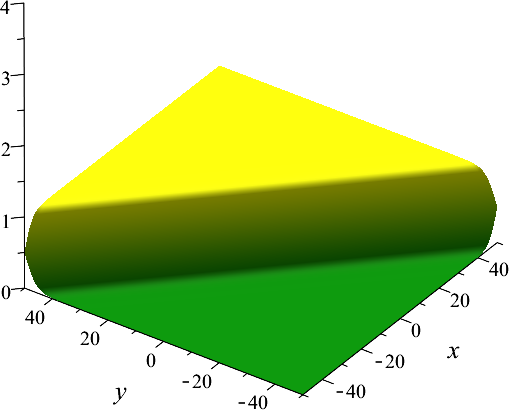
\includegraphics[width=.3\textwidth]{../paper/fig/(3+1)JM-1-soliton.png}    
}
\subfigure[2-孤子解 \label{jm:2-soliton}]{
    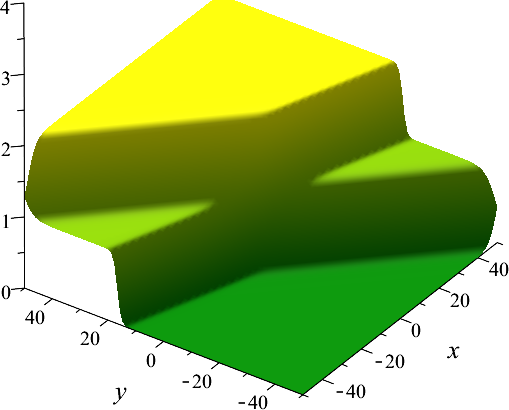
\includegraphics[width=.3\textwidth]{../paper/fig/(3+1)JM-2-soliton.png}
}
\subfigure[3-孤子解 \label{jm:3-soliton}]{
    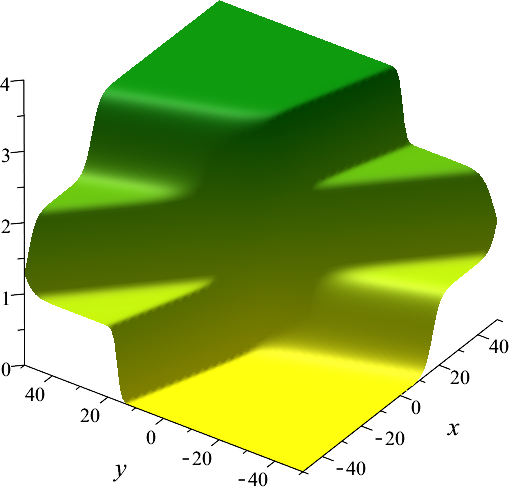
\includegraphics[width=.3\textwidth]{../paper/fig/(3+1)JM-3-soliton.png}
}
\end{figure}
\end{frame}

\begin{frame}
\frametitle{基于$n$孤子解计算呼吸子解}
\begin{columns}
\begin{column}{0.5\textwidth}
算法:
\[
    f_{m-breather}=\conj{f_{(2m)-soliton}} 
\]
\[
    p_{i,j}=p_{i,j+m}^*,~(j=1,2,\cdots,m)
\]
\[
\begin{aligned}
    p_{i,j}&=p_{i,j,RE}+I\cdot p_{i,j,IM}, \\ 
    p_{i,j+m}&=p_{i,j,RE}-I\cdot p_{i,j,IM},
\end{aligned}
\]
\end{column}
\begin{column}{0.5\textwidth}
例子: $m=1,\PS=\bbrace{1,2}$,\\$\xi=k_i(x+p_i y+qz+\omega t)+c$.
\[
\begin{aligned}
    k_1&=k_{1,RE}+I\cdot k_{1,IM} \\ 
    k_2&=k_{1,RE}-I\cdot k_{1,IM} \\
    p_1&=p_{1,RE}-I\cdot p_{1,IM} \\
    p_2&=p_{1,RE}+I\cdot p_{1,IM} \\ 
\end{aligned} 
\]
\end{column}
\end{columns}
\end{frame}

\begin{frame}
\begin{figure}
\setcounter{subfigure}{0}
\subfigure[1-呼吸子解 \label{jm:1-breather}]{
    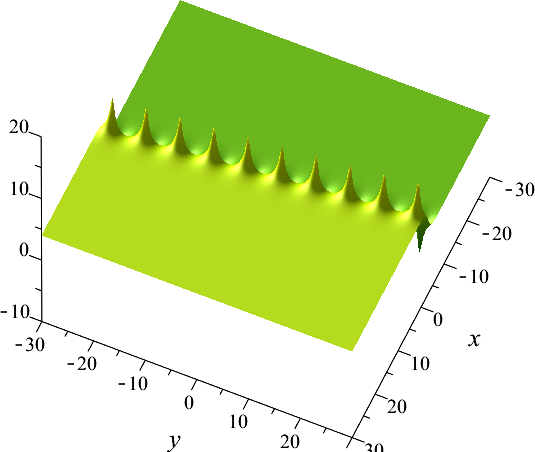
\includegraphics[width=.3\textwidth]{../paper/fig/(3+1)JM-1-breather.png}
}
\subfigure[2-呼吸子解 \label{jm:2-breather}]{
    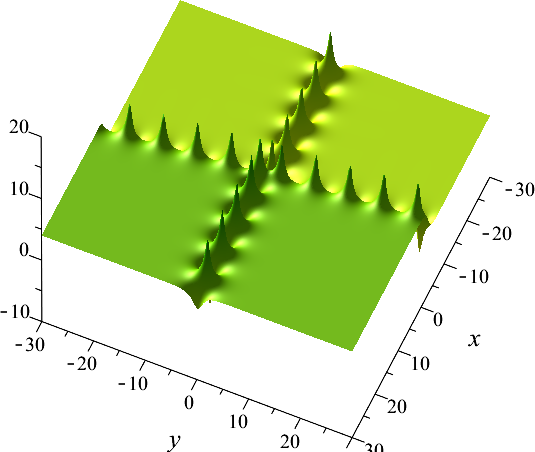
\includegraphics[width=.3\textwidth]{../paper/fig/(3+1)JM-2-breather.png}
}
\subfigure[3-呼吸子解 \label{jm:3-breather}]{
    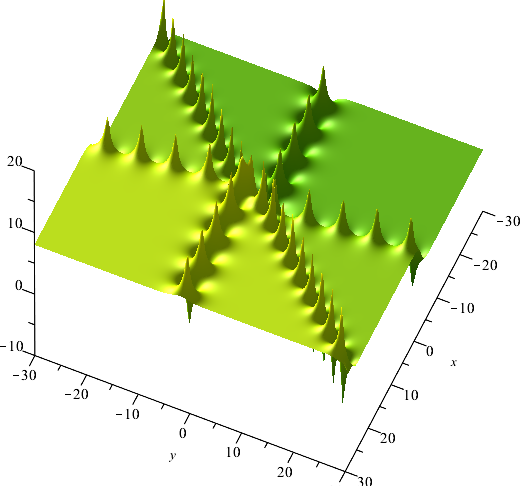
\includegraphics[width=.3\textwidth]{../paper/fig/(3+1)JM-3-breather.png}
}
\subfigure[周期波解 \label{jm:1-periodic}]{
    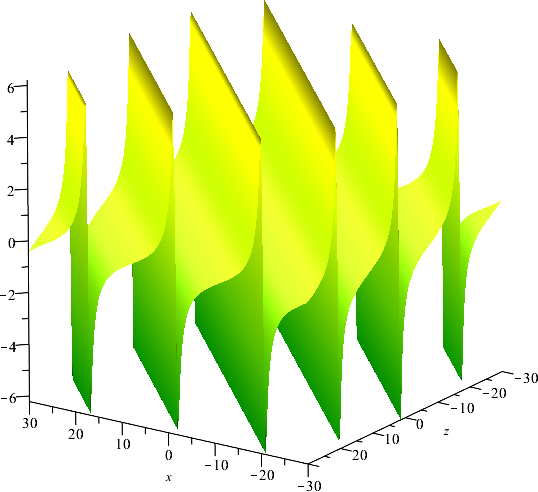
\includegraphics[width=.3\textwidth]{../paper/fig/(3+1)JM-1-periodic.png}
}
\subfigure[孤子-呼吸子相互作用解 \label{jm:soliton-breather}]{
    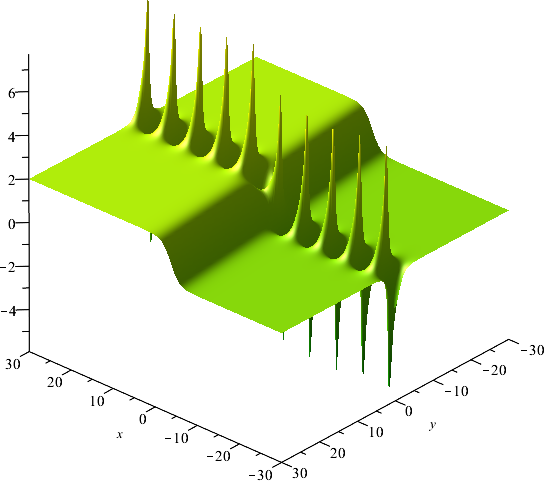
\includegraphics[width=.3\textwidth]{../paper/fig/(3+1)JM-soliton-breather.png}
}
\end{figure}
\end{frame}

\begin{frame}{长极限法与 lump 解}
首先, 令
\begin{equation}
\begin{aligned}
    \xi_i&=k_i\sbrace{x_1+p_ix_2+\cdots+r_ix_n+\omega t}+\xi_i^{(0)},\\
    \eta_i&=\xi_i-\xi_i^{(0)}.
\end{aligned}
\end{equation}
长极限法的关键在于当$k_i,k_j\rightarrow 0$时, 找到这样两个展开:
\begin{equation}
\begin{aligned}
    \exp(\eta_i)&=1+k_i \theta_i+o(k_i), \\ 
    h_{i,j}&=1+k_ik_jb_{i,j}+o(k_i^2+k_j^2),
\end{aligned} \label{lump-expansion}
\end{equation}
其中$o(f)$是Peano余项, 满足$\lim_{f\rightarrow 0}[o(f)/f]=0$.
% \begin{equation*}
% \theta_i=\eval{\frac{\partial \xi_i}{\partial k_i}}{k_i=0}, 
% \end{equation*}
% \begin{equation*}
%     b_{i,j}=\eval{\frac{\partial^2}{\partial k_i\partial k_j}h_{i,j}}{k_i=0,k_j=0}.
% \end{equation*}
\end{frame}

\begin{frame}{计算关键参数}
\begin{columns}
\begin{column}{0.5\textwidth}
关键参数:
\[
\begin{aligned}
    \theta_i &= \eval{\frac{\partial \xi_i}{\partial p_{1,i}}}{p_{1,i}=0}, \\
    b_{i,j}&= \eval{\frac{\partial^2}{\partial p_{1,i}\partial p_{1,j}}h_{i,j}}{p_{1,i}=0,p_{1,j}=0}.
\end{aligned}
\]
\end{column}
\begin{column}{0.5\textwidth}
例子: $\PS=\bbrace{1,2}$
\[
\begin{aligned}
    &\theta_i=\frac{2p_i^2y+(2qz+2x)p_i+3qt}{2p_i}, \\ 
    &b_{i,j}=-\frac{2p_ip_j(p_i+p_j)}{q(p_i-p_j)^2}.
\end{aligned}
\]
\end{column}
\end{columns}
\end{frame}

\begin{frame}
取$\exp\sbrace{\xi_i^{(0)}}=-1$, 并将上述展开代入到($2m$)-孤子解的生成公式中, 可以得到$m$-lump解. 例如对于一个2-孤子解, 我们有 
\begin{equation*}
\begin{aligned}
\Theta_1&=1+\exp(\xi_1)+\exp(\xi_2)+h_{12}\exp(\xi_1+\xi_2) \\ 
&= 1+\exp(\xi_1)+\exp(\xi_2)+(1+k_1k_2b_{12})\exp(\xi_1+\xi_2) +o(k_1 k_2)\\ 
&=(1+\exp(\xi_1))(1+\exp(\xi_2))+k_1k_2b_{12}\exp(\eta_1+\eta_2) +o(k_1 k_2)\\ 
&=(1-(1+k_1\theta_1))(1-(1+k_2\theta_2))+k_1k_2b_{12} +o(k_1 k_2)\\
&=k_1k_2(\theta_1\theta_2+b_{12})+o(k_1 k_2).
\end{aligned}
\end{equation*}
忽略余项后, 又因为$k_1k_2$是一个能够被TPE消除的常数因子, 所以1-lump解的生成公式为
\begin{equation*}
    \Theta_1=\theta_1\theta_2+b_{12}.
\end{equation*}
\end{frame}
\begin{frame}
推广后可得最终的生成公式为:
\[
    f_{m-lump}=\conj{\Theta_m}
\]
\[
\begin{aligned}
    \Theta_m&=\prod_{k=1}^{2m}\theta_k+\frac{1}{2}\sum_{i,j}{b_{i,j}}\prod_{J\neq i,j}{\theta_J}+\frac{1}{2! 2^2}\sum_{i,j,k,l}{b_{i,j}b_{k,l}}\prod_{J\neq i,j,k,l}{\theta_{J}}+\cdots \\
    &+\frac{1}{s!2^s}\sum_{i,j,\cdots,u,v}\underbrace{{b_{i,j}b_{k,l}\cdots b_{u,v}}}_{s}\prod_{J\neq i,j,\cdots, u,v}{\theta_J}+\cdots 
\end{aligned}
\]
例子:
\[
\begin{aligned}
\Theta_1&=\theta_{1}\theta_{2}+b_{12} \\
\Theta_2&=\theta_{1}\theta_{2}\theta_{3}\theta_{4}+b_{12}\theta_{3}\theta_{4}+b_{13}\theta_{2}\theta_{4}+b_{14}\theta_{2}\theta_{3}+b_{23}\theta_{1}\theta_{4}\\
&+b_{24}\theta_{1}\theta_{3}+b_{34}\theta_{1}\theta_{2}+b_{12}b_{34}+b_{13}b_{34}+b_{14}b_{23}
\end{aligned}
\]
\end{frame}

\begin{frame}
重写生成公式
\[
    \Theta_m =\sum_{l=0}^m\sum_{s\in L(l)}\sbrace{\prod_{k=1}^l{b_{s_{2k-1},s_{2k}}}\prod_{p\not\in s}{\theta_p}}
\]
\[
    L(l)=\bbrace{\sbrace{s_1, s_2, \cdots ,s_{2l}}\left|s_{2k}>s_{2k-1},s_{2k+1}>s_{2k-1},s_k\in \bbrace{1,\cdots,2l}\right.}
\]
\begin{itemize}
\item $s_{2k}>s_{2k-1}$ 保证了$b_{i,j}=b_{j,i}$的等价情况只出现一次. 
\item $s_{2k+1}>s_{2k-1}$ 保证了$b_{i,j}$的全排列只出现一次.
\end{itemize}
\end{frame}

\begin{frame}
\small
\[
\renewcommand{\arraystretch}{0.8} 
\begin{array}{l}
\Theta_3=\theta_{{1}}\theta_{{2}}\theta_{{3}}\theta_{{4}}\theta_{{5}}\theta_{{6}}
+b_{{12}}\theta_{{3}}\theta_{{4}}\theta_{{5}}\theta_{{6}}
+b_{{13}}\theta_{{2}}\theta_{{4}}\theta_{{5}}\theta_{{6}}
+b_{{14}}\theta_{{2}}\theta_{{3}}\theta_{{5}}\theta_{{6}}\\
+b_{{15}}\theta_{{2}}\theta_{{3}}\theta_{{4}}\theta_{{6}}
+b_{{16}}\theta_{{2}}\theta_{{3}}\theta_{{4}}\theta_{{5}}
+b_{{23}}\theta_{{1}}\theta_{{4}}\theta_{{5}}\theta_{{6}}
+b_{{24}}\theta_{{1}}\theta_{{3}}\theta_{{5}}\theta_{{6}}\\
+b_{{25}}\theta_{{1}}\theta_{{3}}\theta_{{4}}\theta_{{6}}
+b_{{26}}\theta_{{1}}\theta_{{3}}\theta_{{4}}\theta_{{5}}
+b_{{34}}\theta_{{1}}\theta_{{2}}\theta_{{5}}\theta_{{6}}
+b_{{35}}\theta_{{1}}\theta_{{2}}\theta_{{4}}\theta_{{6}}\\
+b_{{36}}\theta_{{1}}\theta_{{2}}\theta_{{4}}\theta_{{5}}
+b_{{45}}\theta_{{1}}\theta_{{2}}\theta_{{3}}\theta_{{6}}
+b_{{46}}\theta_{{1}}\theta_{{2}}\theta_{{3}}\theta_{{5}}
+b_{{56}}\theta_{{1}}\theta_{{2}}\theta_{{3}}\theta_{{4}}\\
+b_{{12}}b_{{34}}\theta_{{5}}\theta_{{6}}
+b_{{12}}b_{{35}}\theta_{{4}}\theta_{{6}}
+b_{{12}}b_{{36}}\theta_{{4}}\theta_{{5}}
+b_{{12}}b_{{45}}\theta_{{3}}\theta_{{6}}
+b_{{12}}b_{{46}}\theta_{{3}}\theta_{{5}}\\
+b_{{12}}b_{{56}}\theta_{{3}}\theta_{{4}}
+b_{{13}}b_{{24}}\theta_{{5}}\theta_{{6}}
+b_{{13}}b_{{25}}\theta_{{4}}\theta_{{6}}
+b_{{13}}b_{{26}}\theta_{{4}}\theta_{{5}}
+b_{{13}}b_{{45}}\theta_{{2}}\theta_{{6}}\\
+b_{{13}}b_{{46}}\theta_{{2}}\theta_{{5}}
+b_{{13}}b_{{56}}\theta_{{2}}\theta_{{4}}
+b_{{14}}b_{{23}}\theta_{{5}}\theta_{{6}}
+b_{{14}}b_{{25}}\theta_{{3}}\theta_{{6}}
+b_{{14}}b_{{26}}\theta_{{3}}\theta_{{5}}\\
+b_{{14}}b_{{35}}\theta_{{2}}\theta_{{6}}
+b_{{14}}b_{{36}}\theta_{{2}}\theta_{{5}}
+b_{{14}}b_{{56}}\theta_{{2}}\theta_{{3}}
+b_{{15}}b_{{23}}\theta_{{4}}\theta_{{6}}
+b_{{15}}b_{{24}}\theta_{{3}}\theta_{{6}}\\
+b_{{15}}b_{{26}}\theta_{{3}}\theta_{{4}}
+b_{{15}}b_{{34}}\theta_{{2}}\theta_{{6}}
+b_{{15}}b_{{36}}\theta_{{2}}\theta_{{4}}
+b_{{15}}b_{{46}}\theta_{{2}}\theta_{{3}}
+b_{{16}}b_{{23}}\theta_{{4}}\theta_{{5}}\\
+b_{{16}}b_{{24}}\theta_{{3}}\theta_{{5}}
+b_{{16}}b_{{25}}\theta_{{3}}\theta_{{4}}
+b_{{16}}b_{{34}}\theta_{{2}}\theta_{{5}}
+b_{{16}}b_{{35}}\theta_{{2}}\theta_{{4}}
+b_{{16}}b_{{45}}\theta_{{2}}\theta_{{3}}\\
+b_{{23}}b_{{45}}\theta_{{1}}\theta_{{6}}
+b_{{23}}b_{{46}}\theta_{{1}}\theta_{{5}}
+b_{{23}}b_{{56}}\theta_{{1}}\theta_{{4}}
+b_{{24}}b_{{35}}\theta_{{1}}\theta_{{6}}
+b_{{24}}b_{{36}}\theta_{{1}}\theta_{{5}}\\
+b_{{24}}b_{{56}}\theta_{{1}}\theta_{{3}}
+b_{{25}}b_{{34}}\theta_{{1}}\theta_{{6}}
+b_{{25}}b_{{36}}\theta_{{1}}\theta_{{4}}
+b_{{25}}b_{{46}}\theta_{{1}}\theta_{{3}}
+b_{{26}}b_{{34}}\theta_{{1}}\theta_{{5}}\\
+b_{{26}}b_{{35}}\theta_{{1}}\theta_{{4}}
+b_{{26}}b_{{45}}\theta_{{1}}\theta_{{3}}
+b_{{34}}b_{{56}}\theta_{{1}}\theta_{{2}}
+b_{{35}}b_{{46}}\theta_{{1}}\theta_{{2}}
+b_{{36}}b_{{45}}\theta_{{1}}\theta_{{2}}\\
+b_{{12}}b_{{34}}b_{{56}}
+b_{{12}}b_{{35}}b_{{46}}
+b_{{12}}b_{{36}}b_{{45}}
+b_{{13}}b_{{24}}b_{{56}}
+b_{{13}}b_{{25}}b_{{46}}
+b_{{13}}b_{{26}}b_{{45}}\\
+b_{{14}}b_{{23}}b_{{56}}
+b_{{14}}b_{{25}}b_{{36}}
+b_{{14}}b_{{26}}b_{{35}}
+b_{{15}}b_{{23}}b_{{46}}
+b_{{15}}b_{{24}}b_{{36}}
+b_{{15}}b_{{26}}b_{{34}}\\
+b_{{16}}b_{{23}}b_{{45}}
+b_{{16}}b_{{24}}b_{{35}}
+b_{{16}}b_{{25}}b_{{34}} .
\end{array}
\]
\end{frame}

% \begin{frame}{推导关键参数}
% 将$\eta$看作是一个关于$k$的函数, 我们有一维泰勒展开  
% \begin{equation*}
% \begin{aligned}
% \exp(\eta(k))&=\exp(\eta(0))+\eta'(0)\exp(\eta(0))k+o(k)\\ 
% &=1+\eta'(0)k+o(k). 
% \end{aligned}
% \end{equation*}
% 从而, 
% \begin{equation*}
% \theta=\eval{\frac{\partial \eta}{\partial k}}{k=0}=\eval{\frac{\partial \xi}{\partial k}}{k=0}.
% \end{equation*}
% \end{frame}

% \begin{frame}
% 令$h_{i,j}=h(k_i,k_j)$, 根据对称性我们有$h(x,y)=h(y,x)$. 此外, 取$k_2=0$可以将2-孤子解退化为1-孤子解, 所以$h(k_1,0)=1$. 根据对称性, 我们有$h(0,k_2)=1$. 从而, $h(0,0)=1$, 且
% \begin{equation*}
%     h_x(0,0)=\eval{\frac{\partial}{\partial x}h(x,0)}{x=0}=0.
% \end{equation*}
% 类似地, 我们有$h_y(0,0)=h_{xx}(0,0)=h_{yy}(0,0)=0$. 因此, $h(x,y)$在$(0,0)$点的二维泰勒展开为 
% \begin{equation*}
% \begin{aligned}
% h(x,y)&=h(0,0)+h_x(0,0)x+h_y(0,0)y \\ 
% &+\frac{1}{2}\mbrace{h_{xx}(0,0)x^2+2h_{xy}(0,0)xy+h_{yy}(0,0)y^2}+o(x^2+y^2) \\ 
% &=1+h_{xy}(0,0)xy+o(x^2+y^2).
% \end{aligned}
% \end{equation*}
% 从而, 我们得到
% \begin{equation*}
%     b_{i,j}=\eval{\frac{\partial^2}{\partial k_i\partial k_j}h_{i,j}}{k_i=0,k_j=0}.
% \end{equation*}
% \end{frame}



\begin{frame}
\begin{figure}
\setcounter{subfigure}{0}
\centering 
\subfigure[1-lump解 \label{jm:1-lump}]{
    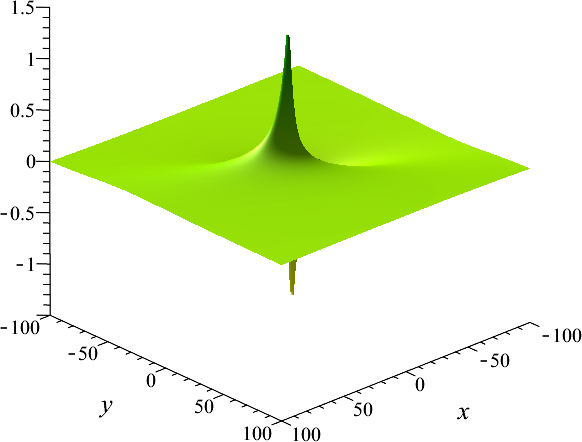
\includegraphics[width=.3\textwidth]{../paper/fig/(3+1)JM-1-lump.png}
}
\subfigure[2-lump解 \label{jm:2-lump}]{
    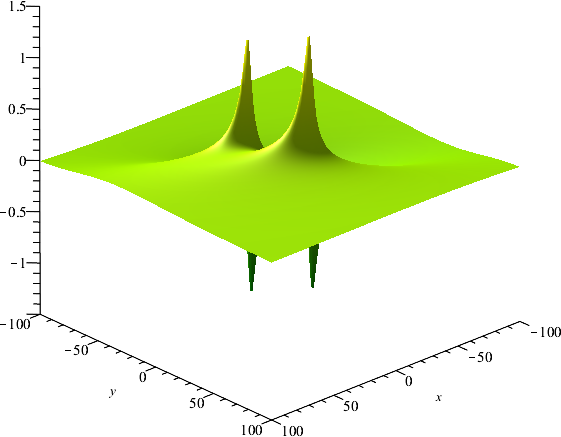
\includegraphics[width=.3\textwidth]{../paper/fig/(3+1)JM-2-lump.png}
}
\subfigure[3-lump解 \label{jm:3-lump}]{
    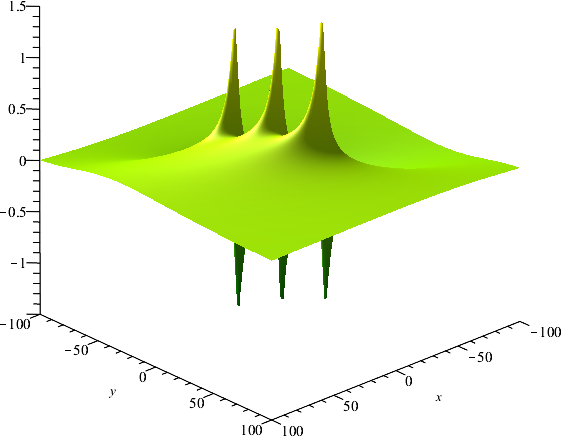
\includegraphics[width=.3\textwidth]{../paper/fig/(3+1)JM-3-lump.png}
}
\subfigure[1-line rogue 解 \label{jm:1-rogue}]{
    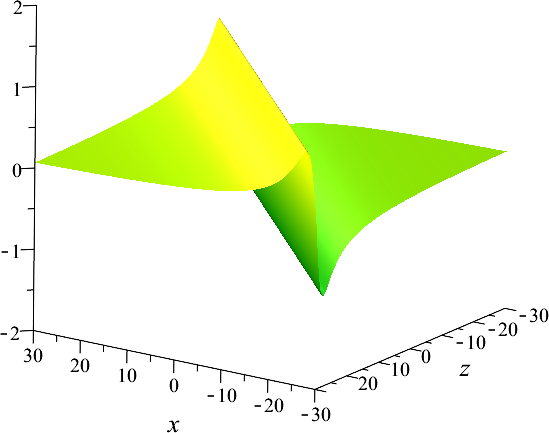
\includegraphics[width=.3\textwidth]{../paper/fig/(3+1)JM-1-rogue.png}
}
\subfigure[2-line rogue 解 \label{jm:2-rogue}]{
    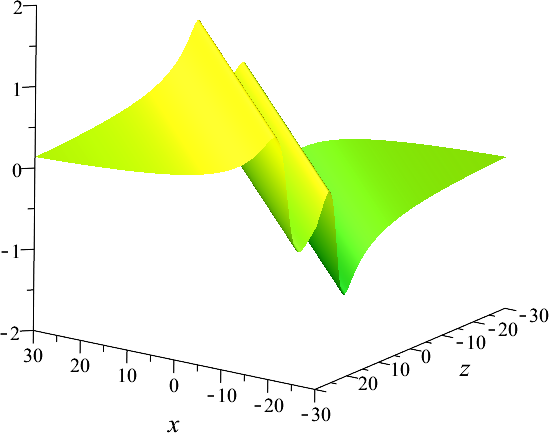
\includegraphics[width=.3\textwidth]{../paper/fig/(3+1)JM-2-rogue.png}
}
\end{figure}
\end{frame}

\begin{frame}
\frametitle{实验与分析}
\footnotesize
\begin{table}[htbp]
\centering
% \caption{测试实例}\label{eqs}
% \renewcommand{\arraystretch}{1.2}
\begin{tabular}{lp{0.7\textwidth}}
\hline
\multicolumn{1}{c}{方程名} & \multicolumn{1}{c}{表达式} \\
\hline
(1+1) KdV & $ u_t+\alpha uu_x+u_{xxx}=0.$\\
(2+1) SK & $5\,{u_{{x}}}^{2}u_{{{\it xx}}}+5\,u_{{x}}u_{{{\it xxxx}}}+5\,u_{{x}}u_{{{\it xy}}}+5\,u_{{{\it xx}}}u_{{{\it xxx}}}+5\,u_{{{\it xx}}}u_{{y}}-u_{{{\it tx}}}+u_{{{\it xxxxxx}}}+5\,u_{{{\it xxxy}}}-5\,u_{{{\it yy}}}=0$.\\
(2+1) KP & $\alpha\,u_{{{\it yy}}}+6\,uu_{{{\it xx}}}+6\,{u_{{x}}}^{2}+u_{{{\it tx}}}+u_{{{\it xxxx}}}=0$.\\
(2+1) BKP-T & $v_{tx}+v_{xxxxxx}-5v_{xxxy}-5v_{yy}+15v_{xx}v_{xxx}+15v_xv_{xxxx}-15v_xv_{xy}-15v_{xx}v_y+45v_x^2v_{xx}=0$. \\
(2+1) CBS & $4\,u_{{x}}u_{{{\it xy}}}+2\,u_{{{\it xx}}}u_{{y}}+u_{{{\it tx}}}+u_{{{\it xxxy}}}=0$.\\
(2+1) CBS-G & $\alpha\,u_{{{\it xy}}}+\beta\,u_{{{\it yy}}}+3\,u_{{x}}u_{{{\it xy}}}+3\,u_{{{\it xx}}}u_{{y}}+u_{{{\it tx}}}+u_{{{\it xxxy}}}=0$.\\
(3+1) CBS & $4\,u_{{x}}u_{{{\it xy}}}+4\,u_{{x}}u_{{{\it xz}}}+2\,u_{{{\it xx}}}u_{{y}}+2\,u_{{{\it xx}}}u_{{z}}+u_{{{\it tx}}}+u_{{{\it xxxy}}}+u_{{{\it xxxz}}}=0$.\\
(3+1) BKP & $-3\,u_{{x}}u_{{{\it xy}}}-3\,u_{{{\it xx}}}u_{{y}}+u_{{{\it ty}}}+3\,u_{{{\it xx}}}-u_{{{\it xxxy}}}+3\,u_{{{\it zz}}}=0$.\\
(3+1) KP & $-6\,uu_{{{\it xx}}}-6\,{u_{{x}}}^{2}+u_{{{\it tx}}}+u_{{{\it xxxx}}}+3\,u_{{{\it yy}}}+3\,u_{{{\it zz}}}=0$.\\
(3+1) NEE & $3\,u_{{{\it xz}}}-2\,u_{{{\it ty}}}-u_{{{\it xxxy}}}+4\,u_{{x}}u_{{y}}+2\,uu_{{{\it xy}}}+2\,u_{{{\it xx}}}\int \!u_{{y}}\,{\rm d}x=0$.\\
(3+1) NEE-T & $2\,v_{{x}}v_{{{\it xxy}}}+4\,v_{{{\it xx}}}v_{{{\it xy}}}+2\,v_{{{\it xxx}}}v_{{y}}-2\,v_{{{\it txy}}}-v_{{{\it xxxxy}}}+3\,v_{{{\it xxz}}}=0$.\\
(3+1) YTSF & $3\,\alpha\,u_{{{\it yy}}}+4\,u_{{x}}u_{{{\it xz}}}+2\,u_{{{\it xx}}}u_{{z}}-4\,u_{{{\it tx}}}+u_{{{\it xxxz}}}=0$.\\
(4+1) Fokas & $u_{tx}-\frac{1}{4}u_{xxxy}+\frac{1}{4}u_{xyyy}+3u_xu_y+3uu_{xy}-\frac{3}{2}u_{wz}=0.$ \\
(4+1) Fokas-T & $au_{t\xi}-\frac{a^3b}{4}u_{\xi\xi\xi\xi}+\frac{ab^3}{4}u_{\xi\xi\xi\xi}+3abu_{\xi}^2+3abuu_{\xi\xi}-\frac{3}{2}u_{wz}=0.$  \\ 
(4+1) Fokas-T-2 & $au_{t\xi}-\frac{a^3b}{4}u_{\xi\xi\xi\xi}+\frac{ab^3}{4}u_{\xi\xi\xi\xi}+3abu_{\xi}^2+3abuu_{\xi\xi}-\frac{3cd}{2}u_{\eta\eta}=0.$\\
\hline
\end{tabular}
\end{table}
\end{frame}
\begin{frame}
\begin{columns}
\begin{column}{0.65\textwidth}
\begin{table}
\centering
\small 
\begin{tabular}{lcccc}
\hline
\multicolumn{1}{c}{方程名} & 1 & 12 & 13 & 123 \\ 
\hline
(1+1)KdV & \tpa\tpb & & & \\
(2+1)BKP-T & \tpa\tpb & \tpa\tpa & & \\
(2+1)KP &\tpa\tpb &\tpa\tpa & & \\
(2+1)SK &\tpa\tpb &\tpa\tpa & & \\
(4+1)Fokas-T-2 &\tpa\tpb &\tpa\tpa & & \\
(2+1)CBS & \tpa\tpb & \tpa\tpb & & \\
(2+1)CBS-G & \tpa\tpb & \tpc\tpc & & \\
(3+1)BKP &\tpa\tpb &\tpa\tpa &\tpa\tpa &\tpc\tpc \\
(3+1)KP &\tpa\tpb &\tpa\tpa &\tpa\tpa &\tpc\tpc \\
(3+1)JM &\tpa\tpb &\tpa\tpa &\tpa\tpb &\tpc\tpc \\
(3+1)NEE-T &\tpa\tpb &\tpa\tpa &\tpa\tpb &\tpc\tpc \\
(3+1)YTSF &\tpa\tpb &\tpa\tpa &\tpa\tpb &\tpb\,\tpb \\
(3+1)CBS &\tpa\tpb &\tpa\tpb &\tpa\tpb &\tpa\tpb \\
(4+1)Fokas-T &\tpa\tpb &\tpa\tpb &\tpa\tpb &\tpc\tpc \\
\hline
\end{tabular}
\end{table}
\end{column}
\begin{column}{0.35\textwidth}
\begin{itemize}
\item `\tpa{}' 表示能够满足原方程.
\item `\tpb{}' 表示不能得到解.
\item `\tpc{}' 表示有解但不满足原方程.
\item 第一个对应3孤子解, 第二个对应2 lump解.
\item 因为有孤子解则一定有呼吸子解, 但不一定有lump解, 所以表中只列出来孤子和lump的对比情况. 
\end{itemize}
\end{column}
\end{columns}
\end{frame}

\begin{frame}
实验结果:
\begin{itemize}
\item $\PS=\bbrace{1}$, 所有方程都有3-孤子解. 
\item $\PS=\ALLP$, 除了两个CBS方程, 所有(2+1)维的方程都有lump解. 
\item $\PS=\ALLP$, (3+1)YTSF方程没有孤子解, 所以不能先取$\PS=\ALLP$, 再取特殊值使得$\PS\subsetneq \ALLP$. 
\item 大部分(3+1)维方程在$\PS=\bbrace{1,2}$或$\PS=\bbrace{1,3}$是才有孤子解和lump解.
\item 孤子解成立是lump解成立的必要条件. 
\end{itemize}
\end{frame}

\begin{frame}{相互作用解}
\begin{enumerate}
\item 推广简单 Hirota 方法
\item 直接代数方法
\end{enumerate}
\end{frame}
